\section{Challenges}
After completing the literature review a variety of potential challenges have been recorded.
Those challenges can be split into two categories, technical and non-technical 

\subsection{Technical Challenges}
Starting with the technical challenges, braille letter spacing is really short allowing only for restricted room between the pins.
This means that the mechanism chosen for controlling the pins as well as the design itself must be compact and take as limited space as possible.
A possible solution for this problem would be using the vertical space as long as the horizontal, potentially stacking components on top of each other to save space. The exact dimension of braille letter according to the UK standard can be seen in figure \ref{fig:BrailleTable} (add reference).
\begin{figure}[h]
\centering
    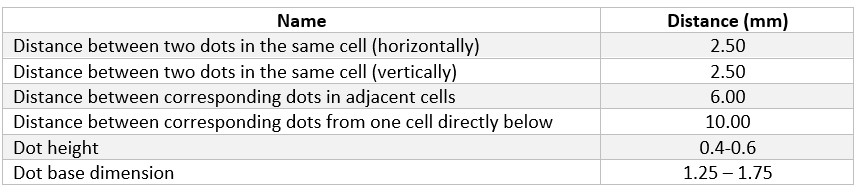
\includegraphics[width=\textwidth]{figures/BrailleDistance Table.jpg}
\caption[Braille Distances Table]{Dimensions of Braille Characters according to UK Standards.}
\label{fig:BrailleTable}
\end{figure}

Additionally, the final device must be able to provide an acceptable refresh rate for the letters so that the reading experience for the users is as smooth as possible without any disruptions for loading time. Given that the average braille reader is able of reading 120-150 words per minute or approximately 7.5 characters per ssecond (reference number 2), each letter should be able to refresh in 0.13 seconds approximately
A potential get-around for this issue would be to for the device to be able to generate more than one letter at a time in a horizontal line.
By allowing each letter to be controlled independently, the letters can change progressively as the reader moves to the next letter allowing this way for little to no downtime and providing us with more time for refreshing the previous letters. Even just using two letters effectively doubles the available time for refresh of each individual character.
 

\subsection{Non-Technical Challenges}
As far as non technical challenges are concerned there are two main areas of interest.
First is the training that will be required for the users to familiarize with the device and second is the marketing of the device.
Given that a substantial proportion of visually impaired people and an even greater proportion of deafblind people belong to the elder population, familiarising with the device is going to be challenging.

Additionally, in the case of deafblind individuals, voice instructions cannot be used during the training process.
To get around those issues, firstly all instructions will be provided both in Braille and audio format and secondly there will be training sessions provided to the caretakers/personnel that works with such individuals in order to be allow them to assist in the training process of the user and make this transition as smooth as possible.
A similar process can be used for the marketing of the device.
By familiarizing organizations such as the RNIB and people working with visually impaired individuals about our product, and explaining the advantages it offers compare to the existing solutions, we can indirectly reach our audience much more effective than by ads. Finally, by promoting the final product to humanitarian organizations of global range, we can expand its target group to third word countries to be used as a tool for teaching braille. 
 